\documentclass{beamer}
\usepackage[utf8]{inputenc}
\usepackage[T1]{fontenc}
\usepackage{mathabx}
\usepackage{mathpazo}
\usepackage{eulervm}
\usepackage{natbib}
\usepackage{tikz}


%% Load the markdown package
\usepackage[citations,footnotes,definitionLists,hashEnumerators,smartEllipses,tightLists=false,pipeTables,tableCaptions,hybrid]{markdown}

%%begin novalidate
\markdownSetup{rendererPrototypes={
 link = {\href{#2}{#1}},
 headingOne = {\section{#1}},
 headingTwo = {\subsection{#1}},
 headingThree = {\begin{frame}\frametitle{#1}},
 headingFour = {\begin{block}{#1}},
 horizontalRule = {\end{block}}
}}
%%end novalidate

\usetheme{Dresden}
\usefonttheme{serif}
\usecolortheme{rose}

% \setbeamertemplate{navigation symbols}{}
% \setbeamertemplate{footline}[frame number]

\title{Studying the NEXUS Presentation}
\titlegraphic{
\includegraphics[width=2cm]{Images/GTLogoSeal_Navy copy.png}
}
\author{Ethan Masters}
\date{August 2, 2022}
\institute{Georgia Institute of Technology}

\begin{document}


\maketitle

\frame{\tableofcontents}


\section{Introduction}
\begin{frame}{The Energy-Climate-Security Nexus}
    \begin{columns}
        \column{0.65\textwidth}
        \begin{itemize}
            \item Climate change necessitates a shift toward sustainable energy sources.
            \item Nuclear energy is positioned as a \textbf{low-carbon solution} but introduces geopolitical and security risks.
            \item This research examines the interplay between \textbf{clean energy, security, and global climate policies}.
        \end{itemize}
        
        \column{0.35\textwidth}
        \centering
        
\includegraphics[width=\textwidth]{Images/gt-seal_0.png} 
    \end{columns}
\end{frame}


\section{Methodology}
\begin{frame}{Research Approach}
    \begin{itemize}
        \item \textbf{Comprehensive Literature Review}: Peer-reviewed journals, government reports, and academic papers.
        \item \textbf{Historical Scope}: Research limited to time of this study (2022).
        \item \textbf{Leximancer Analysis}: Concept mapping to identify thematic connections.
    \end{itemize}
\end{frame}


\begin{frame}{Concept Mapping: Leximancer Analysis}
    \begin{columns}
        \column{0.5\textwidth}
        \begin{itemize}
            \item Identified \textbf{key themes}:
            \begin{itemize}
                \item \textbf{Nuclear Energy} as a central policy issue.
                \item Connections between \textbf{energy policy, climate mitigation, and security}.
                \item Geopolitical influences from \textbf{Russia, China, and the U.S.}.
            \end{itemize}
        \end{itemize}
        
        \column{0.5\textwidth}
        \centering
        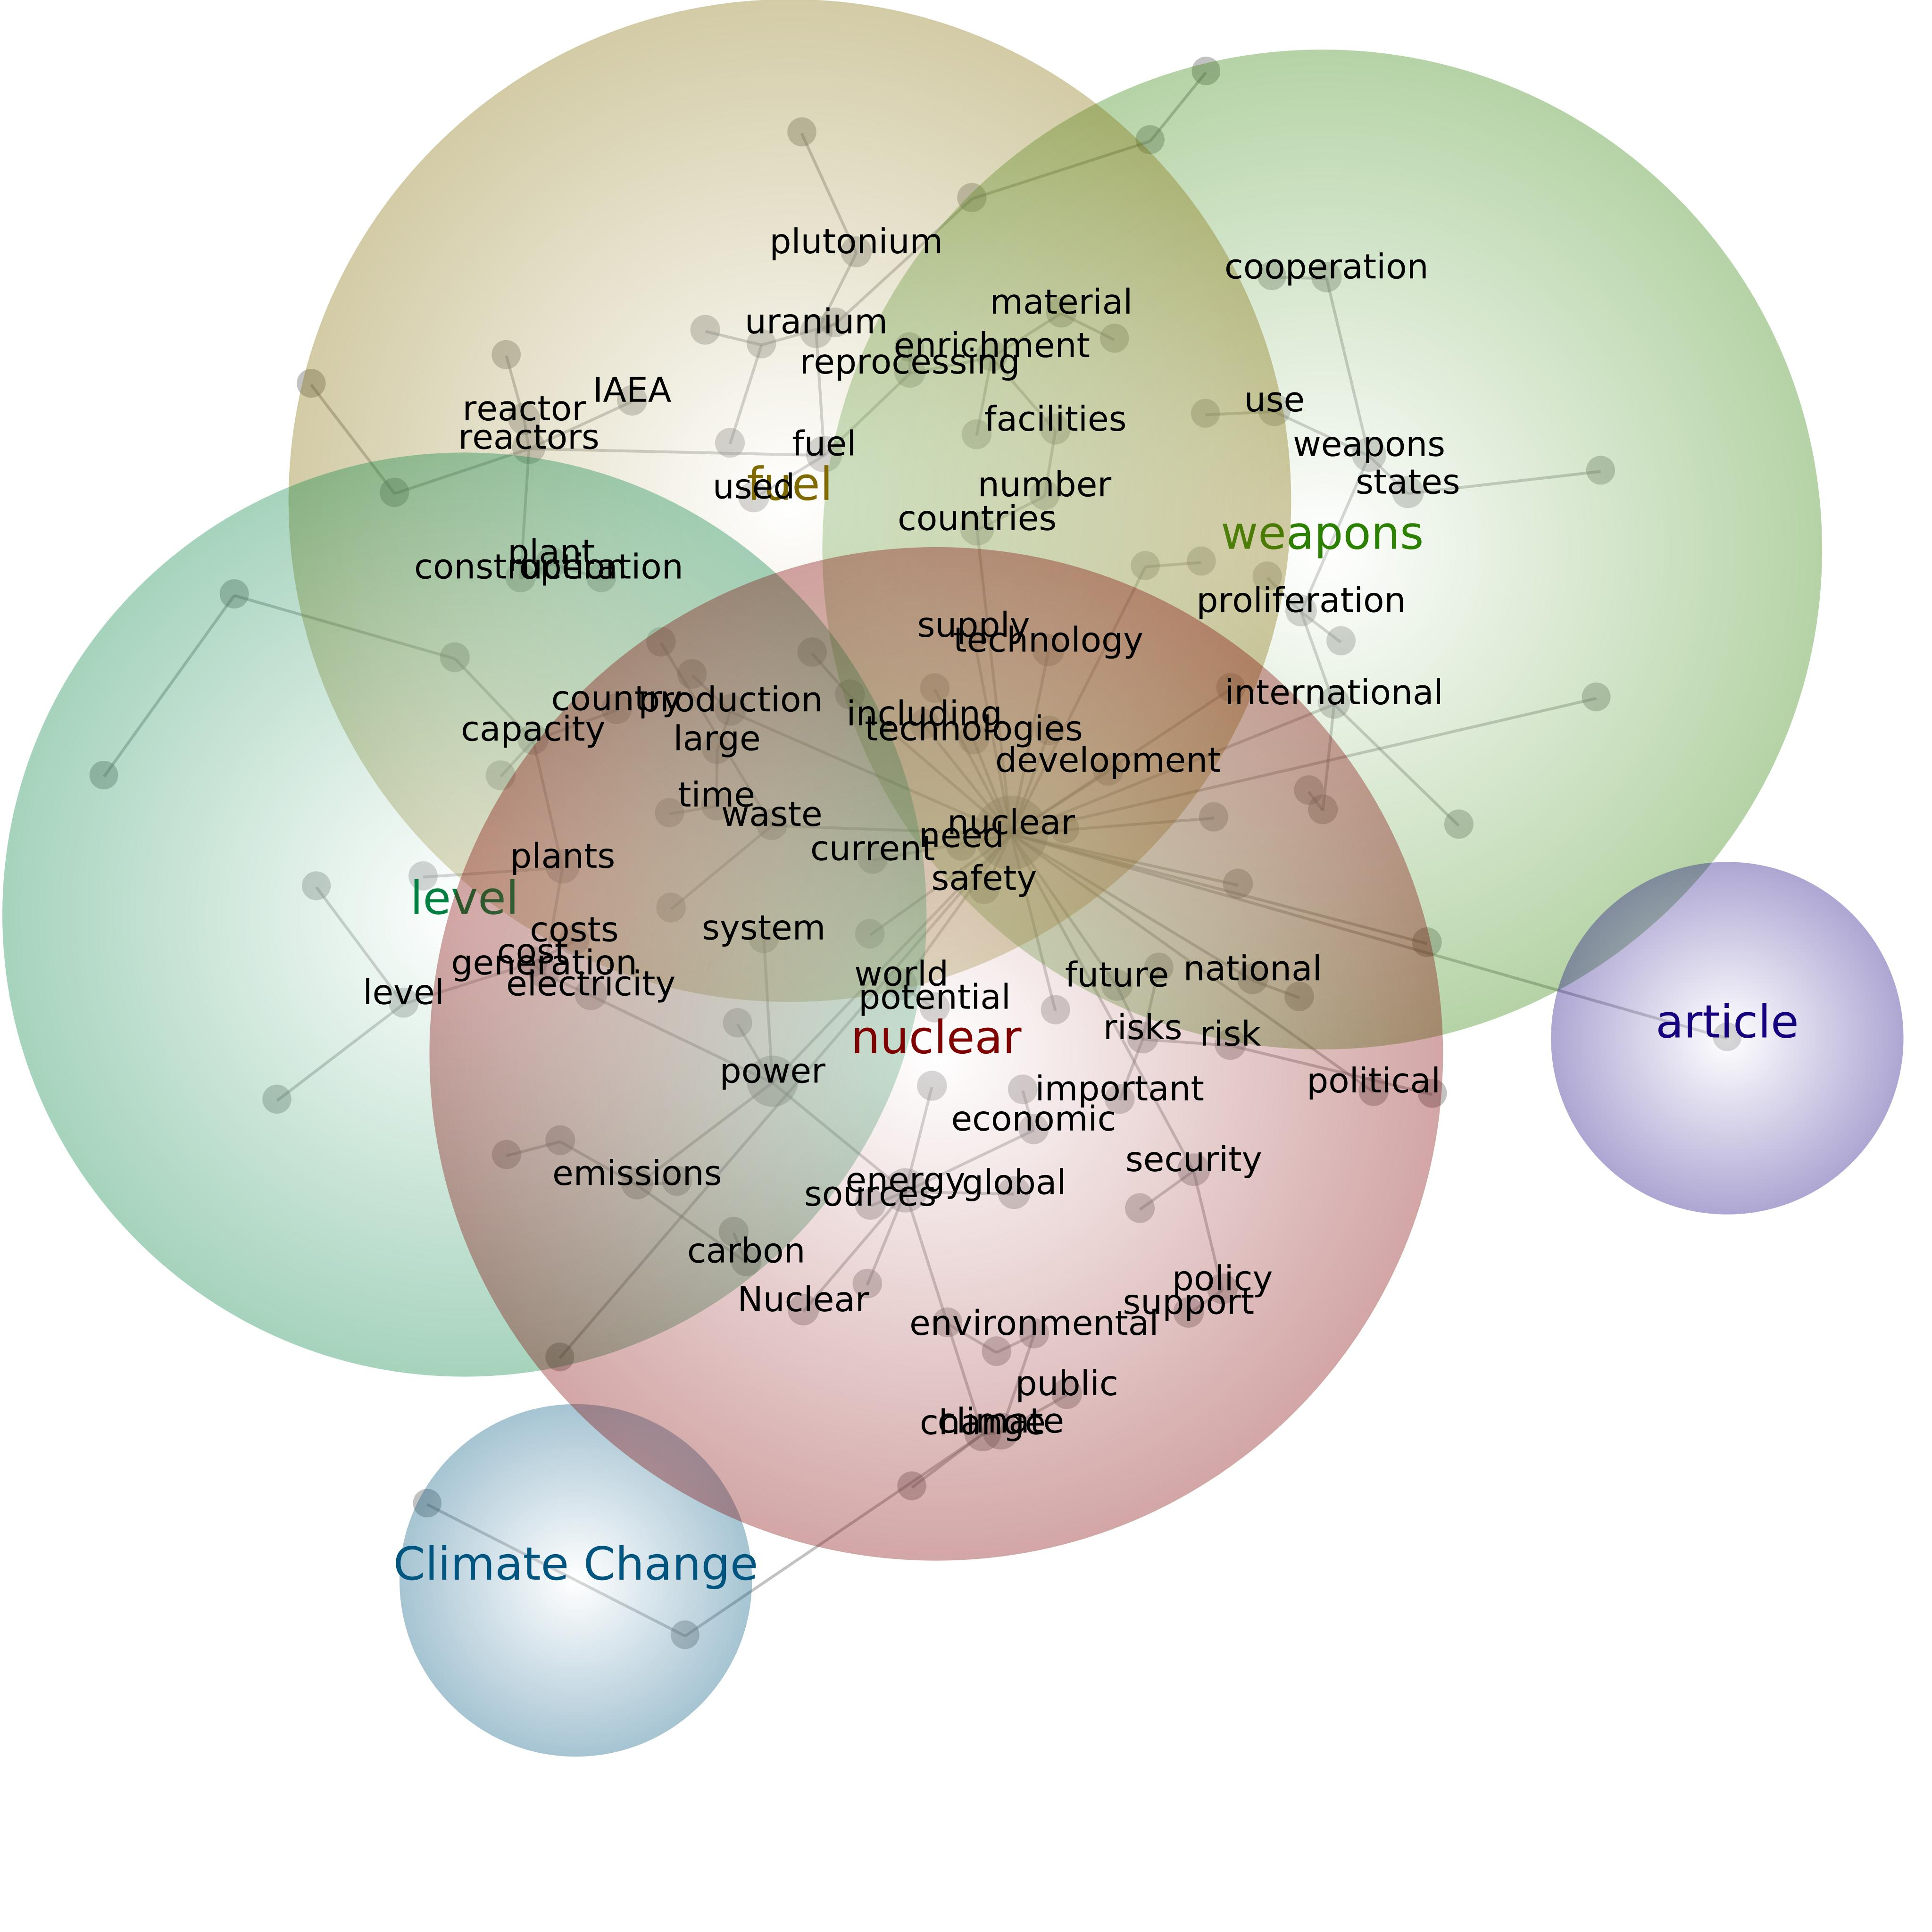
\includegraphics[width=0.9\textwidth]{Images/E Nexus-concept-map.jpeg} % Insert Leximancer concept map
    \end{columns}
\end{frame}


\section{Nuclear Energy in Climate Mitigation}
\begin{frame}{Nuclear Energy: A Decarbonization Tool}
    \begin{itemize}
        \item Nuclear power is a \textbf{stable, low-carbon} energy source.
        \item Supports renewable energy by \textbf{balancing intermittency} in the grid.
        \item Small Modular Reactors (\textbf{SMRs}) are promising but face economic hurdles \cite{DUFFEY2005535}.
    \end{itemize}
\end{frame}


\begin{frame}{Challenges to Nuclear Expansion}
    \begin{itemize}
        \item \textbf{Economic Barriers}: High capital investment, long construction timelines \cite{KESSIDES2012185}.
        \item \textbf{Public Opposition}: Safety concerns, nuclear waste storage, and disaster risk \cite{CORNER20114823}.
        \item \textbf{Competing Renewable Costs}: Wind and solar prices continue to fall, challenging nuclear's viability \cite{LOVINS2022107122}.
    \end{itemize}
\end{frame}


\section{Nuclear Energy and Security}
\begin{frame}{Geopolitical Considerations}
    \begin{itemize}
        \item Civilian nuclear programs create \textbf{dependency} on supplier states.
        \item Russia and China \textbf{dominate nuclear exports}, leveraging contracts for geopolitical influence \cite{Nguyen}.
        \item The U.S. faces declining influence in the global nuclear market.
    \end{itemize}
\end{frame}


\begin{frame}{Proliferation Risks}
    \begin{itemize}
        \item \textbf{Dual-use technology}: Civilian programs can serve as cover for weapons development.
        \item Nuclear expansion increases risk of \textbf{covert weapons proliferation}.
        \item Strengthening \textbf{IAEA and NPT} safeguards is critical \cite{Goldschmidt2010multilateral}.
    \end{itemize}
\end{frame}


\section{Public Perception and Policy}
\begin{frame}{Public Opinion on Nuclear Energy}
    \begin{itemize}
        \item \textbf{Public opinion is divided}: Nuclear is viewed as both a solution and a risk.
        \item Safety, trust, and \textbf{media framing} influence policy support \cite{Doyle}.
        \item Historical opposition shapes national nuclear policies.
    \end{itemize}
\end{frame}


\section{Policy Recommendations}
\begin{frame}{Strengthening Governance}
    \begin{itemize}
        \item \textbf{Strengthen IAEA oversight}: Improve global nuclear monitoring.
        \item \textbf{Fuel Security}: Develop \textbf{multinational} fuel-cycle initiatives to mitigate risks.
        \item \textbf{Investment in Advanced Reactors}: Focus on \textbf{proliferation-resistant} designs.
        \item \textbf{Public Engagement}: Increase transparency to build public trust.
    \end{itemize}
\end{frame}


\section{Conclusion}
\begin{frame}{Key Takeaways}
    \begin{itemize}
        \item Nuclear power offers \textbf{low-carbon energy}, but governance is essential.
        \item Proliferation risks and \textbf{geopolitical complexities} influence expansion.
        \item Policy decisions will determine if nuclear energy advances decarbonization without increasing security risks.
    \end{itemize}
\end{frame}


\begin{frame}[allowframebreaks]{References}
    \bibliographystyle{plainnat}
    \bibliography{references}
\end{frame}


\begin{frame}
    \centering
    \textbf{Thank You!} \\
    Questions?
\end{frame}

\end{document}